\documentclass{beamer}

\usepackage{multicol}
\usepackage{wrapfig}

\definecolor{bostonuniversityred}{rgb}{0.8, 0.0, 0.0}

\newsavebox{\authbox}
\sbox{\authbox}{%
\centering
\begin{minipage}{0.45\linewidth}
\vspace{0.5cm}
\centering\normalsize
Candidate: \par
Davide Peron
\end{minipage}
\hfill
\begin{minipage}{0.45\linewidth}
\vspace{0.5cm}
\centering\normalsize
Supervisor: \par
Prof. Michele Zorzi\\ \vspace{0.5cm}
Co-supervisor: \par
Marco Giordani
\end{minipage}
}

\usetheme{Madrid}
\usecolortheme{beaver}
\graphicspath{{./figures/}}

% \defbeamertemplate*{title page}{customized}[1][]
% {
%   \usebeamerfont{title}\inserttitle\par
%   \usebeamerfont{subtitle}\usebeamercolor[fg]{subtitle}\insertsubtitle\par
%   \bigskip
%   \usebeamerfont{author}\insertauthor\par
%   \usebeamerfont{institute}\insertinstitute\par
%   \usebeamerfont{date}\insertdate\par
%   \usebeamercolor[fg]{titlegraphic}\inserttitlegraphic
% }

\newcommand{\lenitem}[2][.45\linewidth]{\parbox[t]{#1}{\strut #2\strut}}

\setbeamertemplate{caption}[numbered]
\setbeamertemplate{itemize item}{\color{bostonuniversityred}$\bullet$}
\makeatother
\setbeamertemplate{footline}
{
  \leavevmode%
  \hbox{%
  \begin{beamercolorbox}[wd=.2\paperwidth,ht=2.25ex,dp=1ex,center]{author in head/foot}%
    \usebeamerfont{author in head/foot}\insertshortauthor
  \end{beamercolorbox}%
  \begin{beamercolorbox}[wd=.8\paperwidth,ht=2.25ex,dp=1ex,center]{title in head/foot}%
    \usebeamerfont{title in head/foot}\insertshorttitle\hspace*{3em}
    % \insertframenumber{} / \inserttotalframenumber\hspace*{1ex}
  \end{beamercolorbox}}%
  \vskip0pt%
}
\makeatletter
\setbeamertemplate{navigation symbols}{}

\AtBeginSection[]{
  \begin{frame}
  \vfill
  \centering
  \begin{beamercolorbox}[sep=8pt,center,shadow=true,rounded=true]{title}
    \usebeamerfont{title}\insertsectionhead\par%
  \end{beamercolorbox}
  \vfill
  \end{frame}
}

\title{Interface Selection in 5G Vehicular Networks}
\author[Davide Peron]{\usebox{\authbox} \vspace{1cm}}
\date{\small October 8, 2018}
\institute[Unimib]{Università degli studi di Padova}
\titlegraphic{%
	\vspace{-2cm}
	\hspace{0.4cm}
   	
\includegraphics[width=0.18\linewidth]{logoUnipd.png}\hspace*{6cm}~%
   	
\includegraphics[width=0.25\linewidth]{logoDei.png}%
   }


\begin{document}

	\maketitle

	\begin{frame}{Table of contents}
		\tableofcontents
	\end{frame}


	\section{Introduction}

	\begin{frame}{Introduction}
		With the introduction of 5G cellular networks, vehicular networks will be used for safety and infotainment applications. \vspace{.5em}

		\begin{itemize}
			\item \textbf{Safety Applications : } applications to increase vehicle safety on the roads and to reduce the number of accidents. \\ Mainly Vehicle-to-Vehicle communication at low datarates.
			\item \textbf{Non-Safety Applications : } applications to provide road users with information, advertisements and entertainment during their journey. \\ Mainly Vehicle-to-Infrastructure communication at extremely high datarates.
		\end{itemize}
	\end{frame}

	\begin{frame}{Introduction}
		Applications with different requirements have to be handled by different technologies.\\ \vspace{.5em}
		Nowadays technologies cannot support the performance required by Non-Safety Applications\\ \vspace{.5em}
		mmWaves work above 10 GHz and can ensure very high throughput and low latency, but suffer from high blockage sensitivity \\ \vspace{.5em}
		Interface selection techniques using other technologies (such as LTE) are needed to support mmWaves when they did not work.
	\end{frame}

	\begin{frame}{Introduction}
		\textbf{Contribution:} Comparison of mmWaves with LTE and IEEE 802.11p/WAVE through NS3 End-to-End full stack simulations to enable interface selection techniques in future 5G vehicular networks\\ \vspace{1cm}
		Two type of communication have been compared: \vspace{.5em}
		\begin{itemize}
			\item Vehicle-to-Vehicle (V2V) communication using IEEE 802.11p/WAVE\vspace{.5em}
			\item Vehicle-to-Infrastructure (V2I) using LTE and mmWaves \vspace{.5em}
		\end{itemize}
	\end{frame}

	\section{Simulation settings and scenarios}

	\subsection{Vehicle-to-Vehicle scenario}

	\begin{frame}{V2V Scenario}
		\begin{itemize}
			\item IEEE 802.11p has been used given its major use in unstructured and self organized networks
			\item 2 vehicles in Line-of-Sight share data using UDP\vspace{.5em}
			\item The vehicles are not moving
			\item Constant distance ranging from 2 meters to 160 meters\vspace{.5em}
			\item Datarates simulated:  $0.01 ~Mbps$, $1 ~Mbps$, $10 ~Mbps$, $100 ~Mbps$, $1000 ~Mbps$
		\end{itemize}
	\end{frame}

	% \begin{frame}{V2V Scenario}
	% 	\begin{itemize}
	% 		\item \textbf{Channel capacity: } $6 ~Mbps$\vspace{.5em}
	% 		\item \textbf{Bandwidth: } 10MHz\vspace{.5em}
	% 		\item \textbf{Carrier frequency: } 5.875 GHz
	% 		\item \textbf{Application data rates simulated: } $10 ~kbps$, $1 ~Mbps$, $10 ~Mbps$, $100 ~Mbps$, $1000 ~Mbps$
	% 		\item \textbf{Packet Size: } 1000 bytes
	% 	\end{itemize}
	% \end{frame}

	\subsection{Vehicle-to-Infrastructure scenario}

	\begin{frame}{V2I Scenario}
		\vspace{-1cm}
		\mbox{}\hfill\raisebox{-\height}[0pt][0pt]{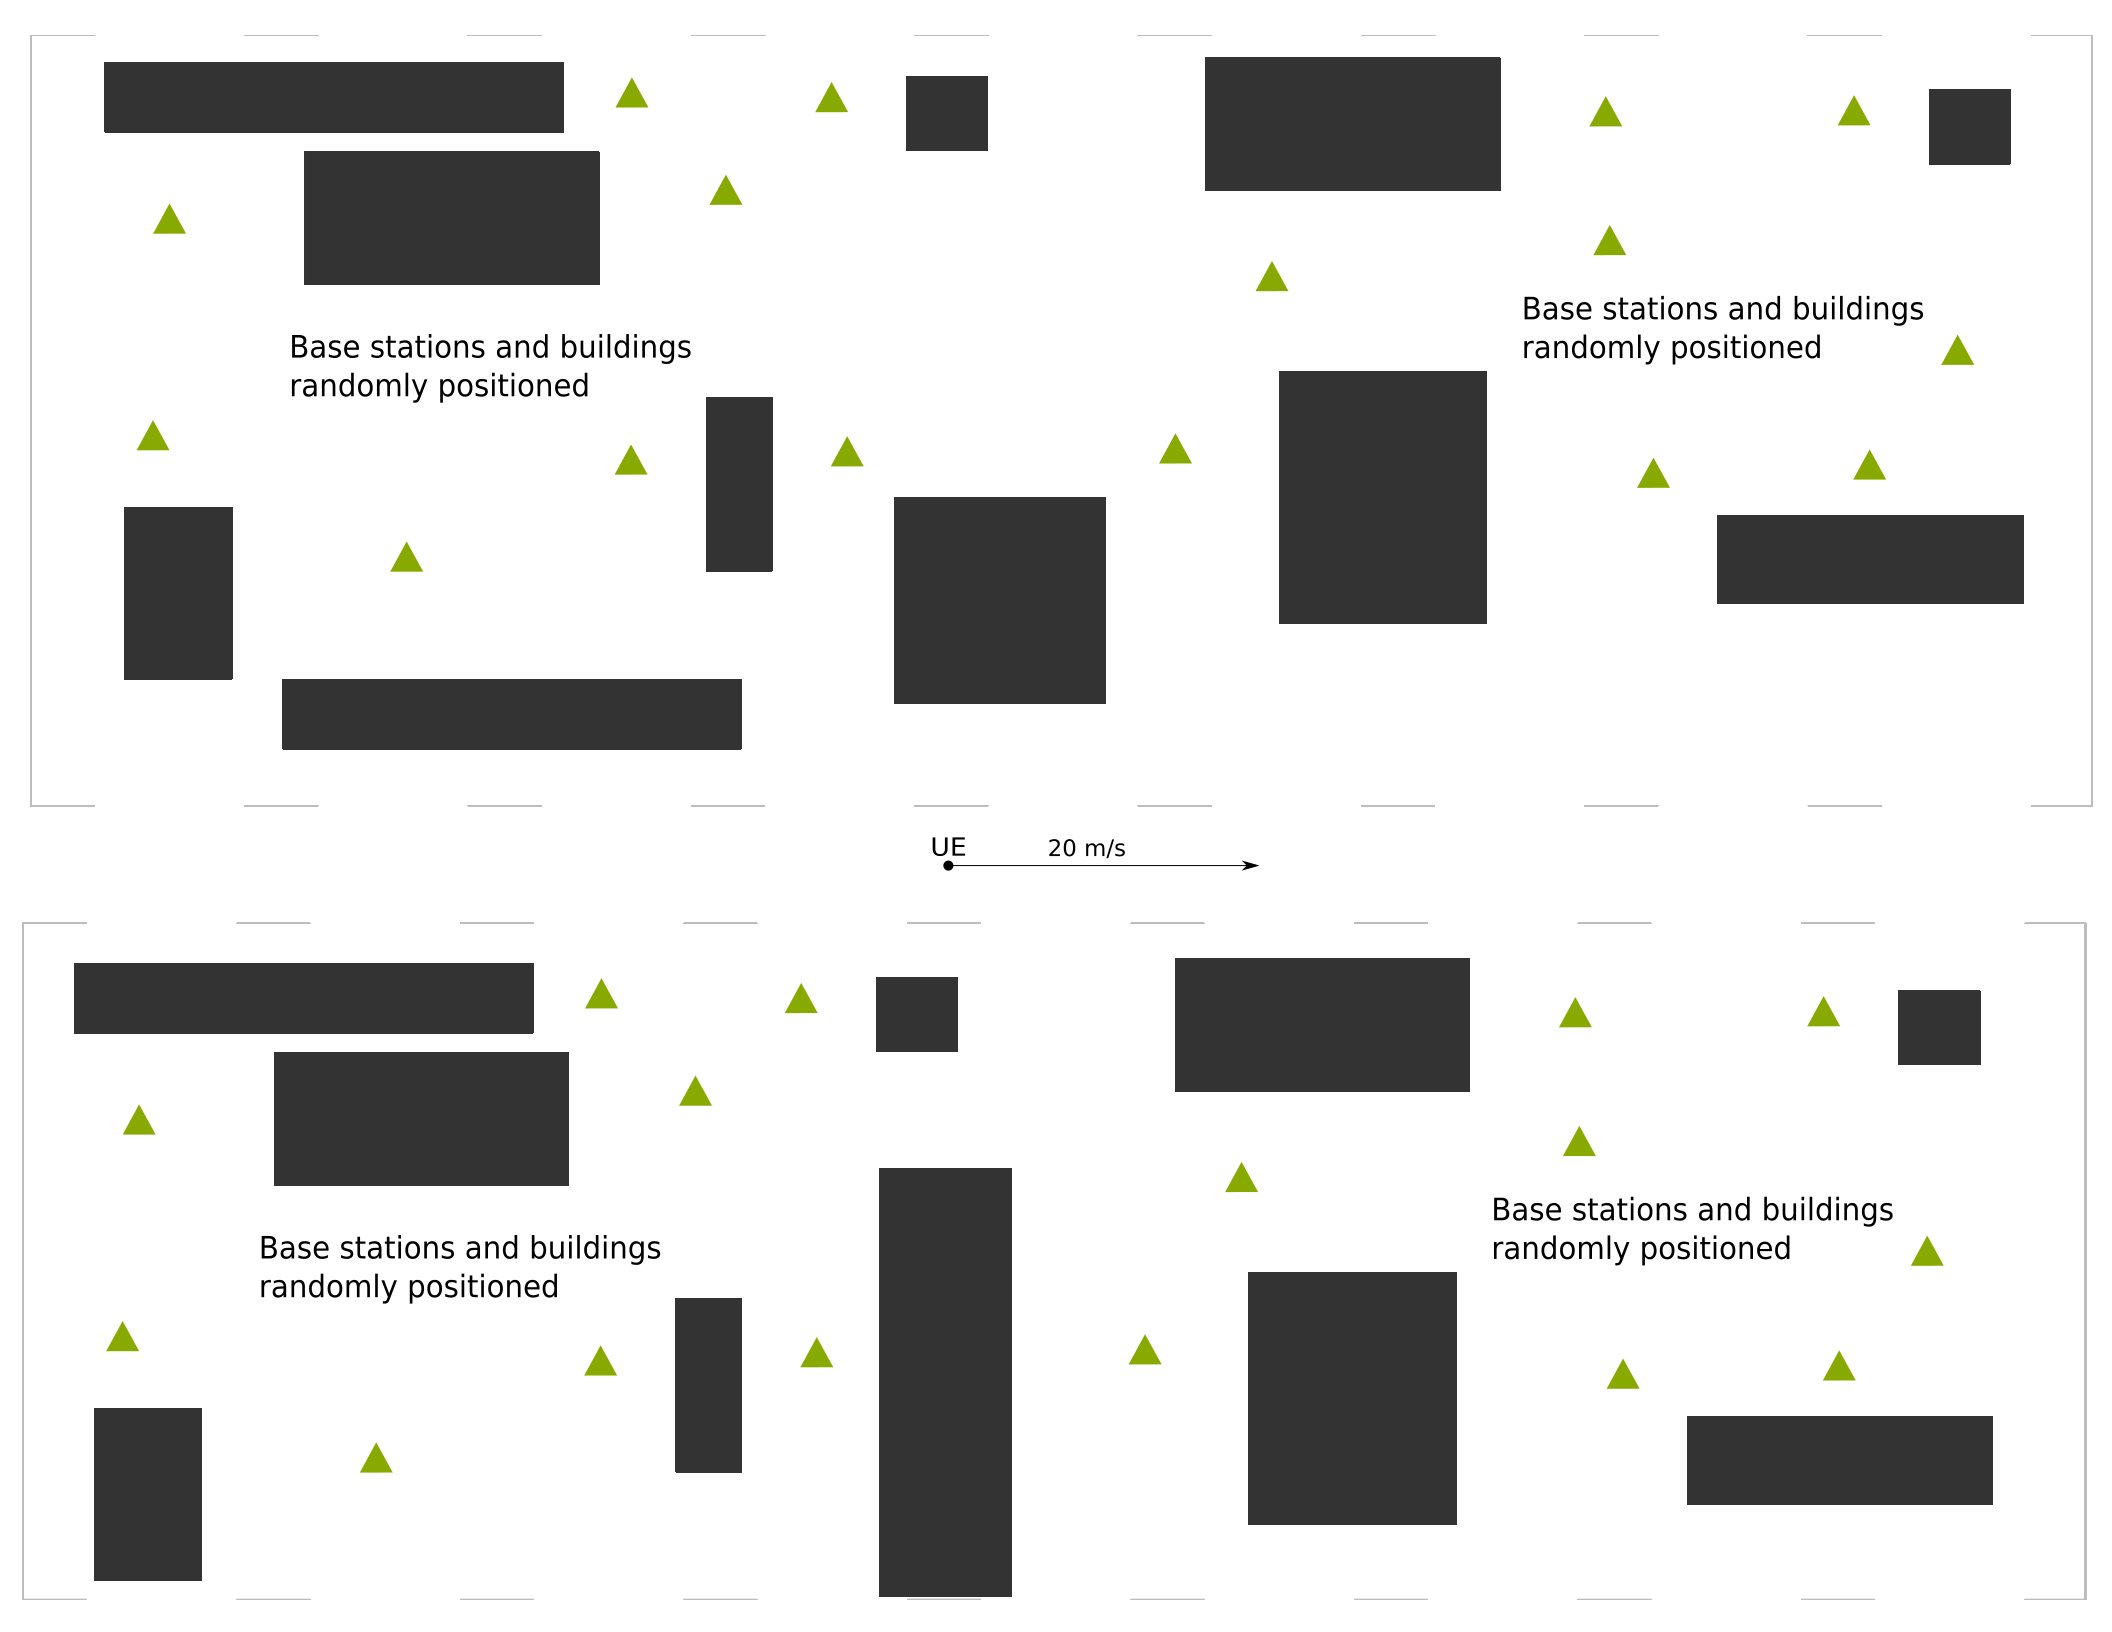
\includegraphics[width=.47\linewidth]{scenario}}
		\begin{itemize}
			\item \lenitem{LTE and mmWaves have been used separately}
			\item \lenitem{Buildings and base stations are randomly deployed in the simulated area} 
			\item \lenitem{A vehicle receives data from a base station using UDP\vspace{.5em}}
			\item The vehicle speed is 20 m/s
			\item Base stations density ranges from 4 to 30 base stations/km$^2$ 
			\item Datarates simulated: $1 ~Mbps$, $10 ~Mbps$, $100 ~Mbps$, $1000 ~Mbps$
		\end{itemize}
		% \begin{wrapfigure}{R}{0.3\textwidth}
		% 	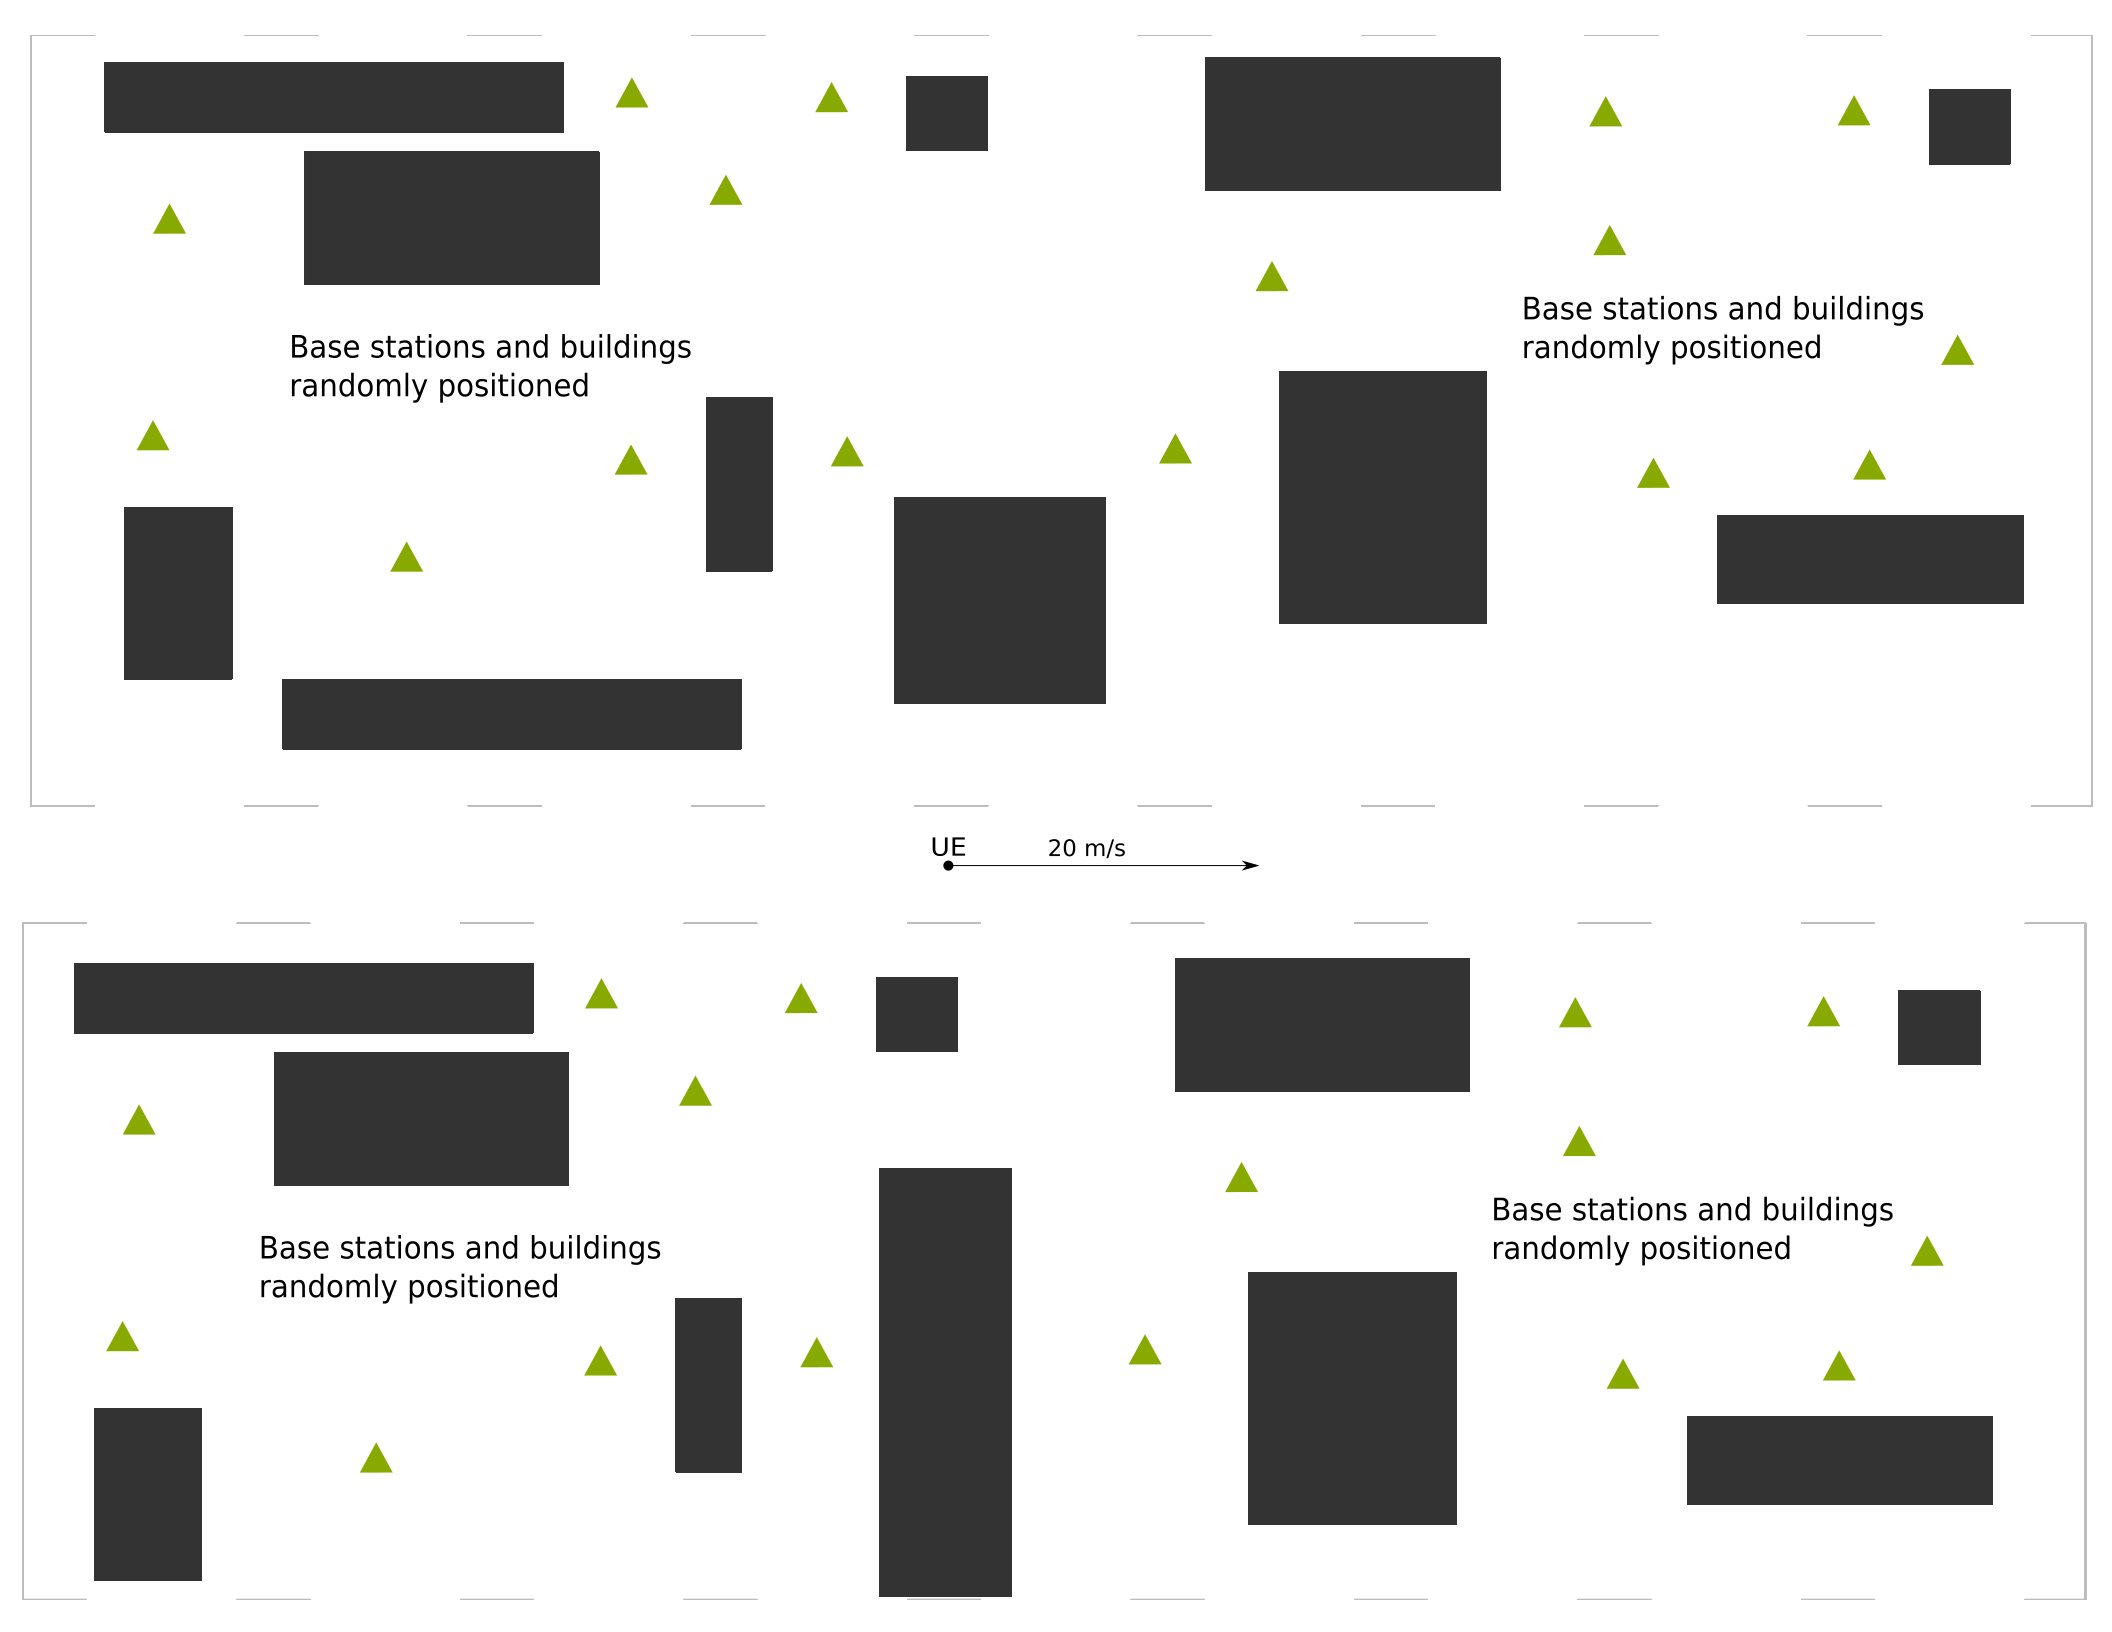
\includegraphics[scale=0.1]{scenario}
		% \end{wrapfigure}
	\end{frame}

	% \begin{frame}{V2I Scenario}
	% 	\begin{figure}
	% 		\vspace{-0.1in}
	% 		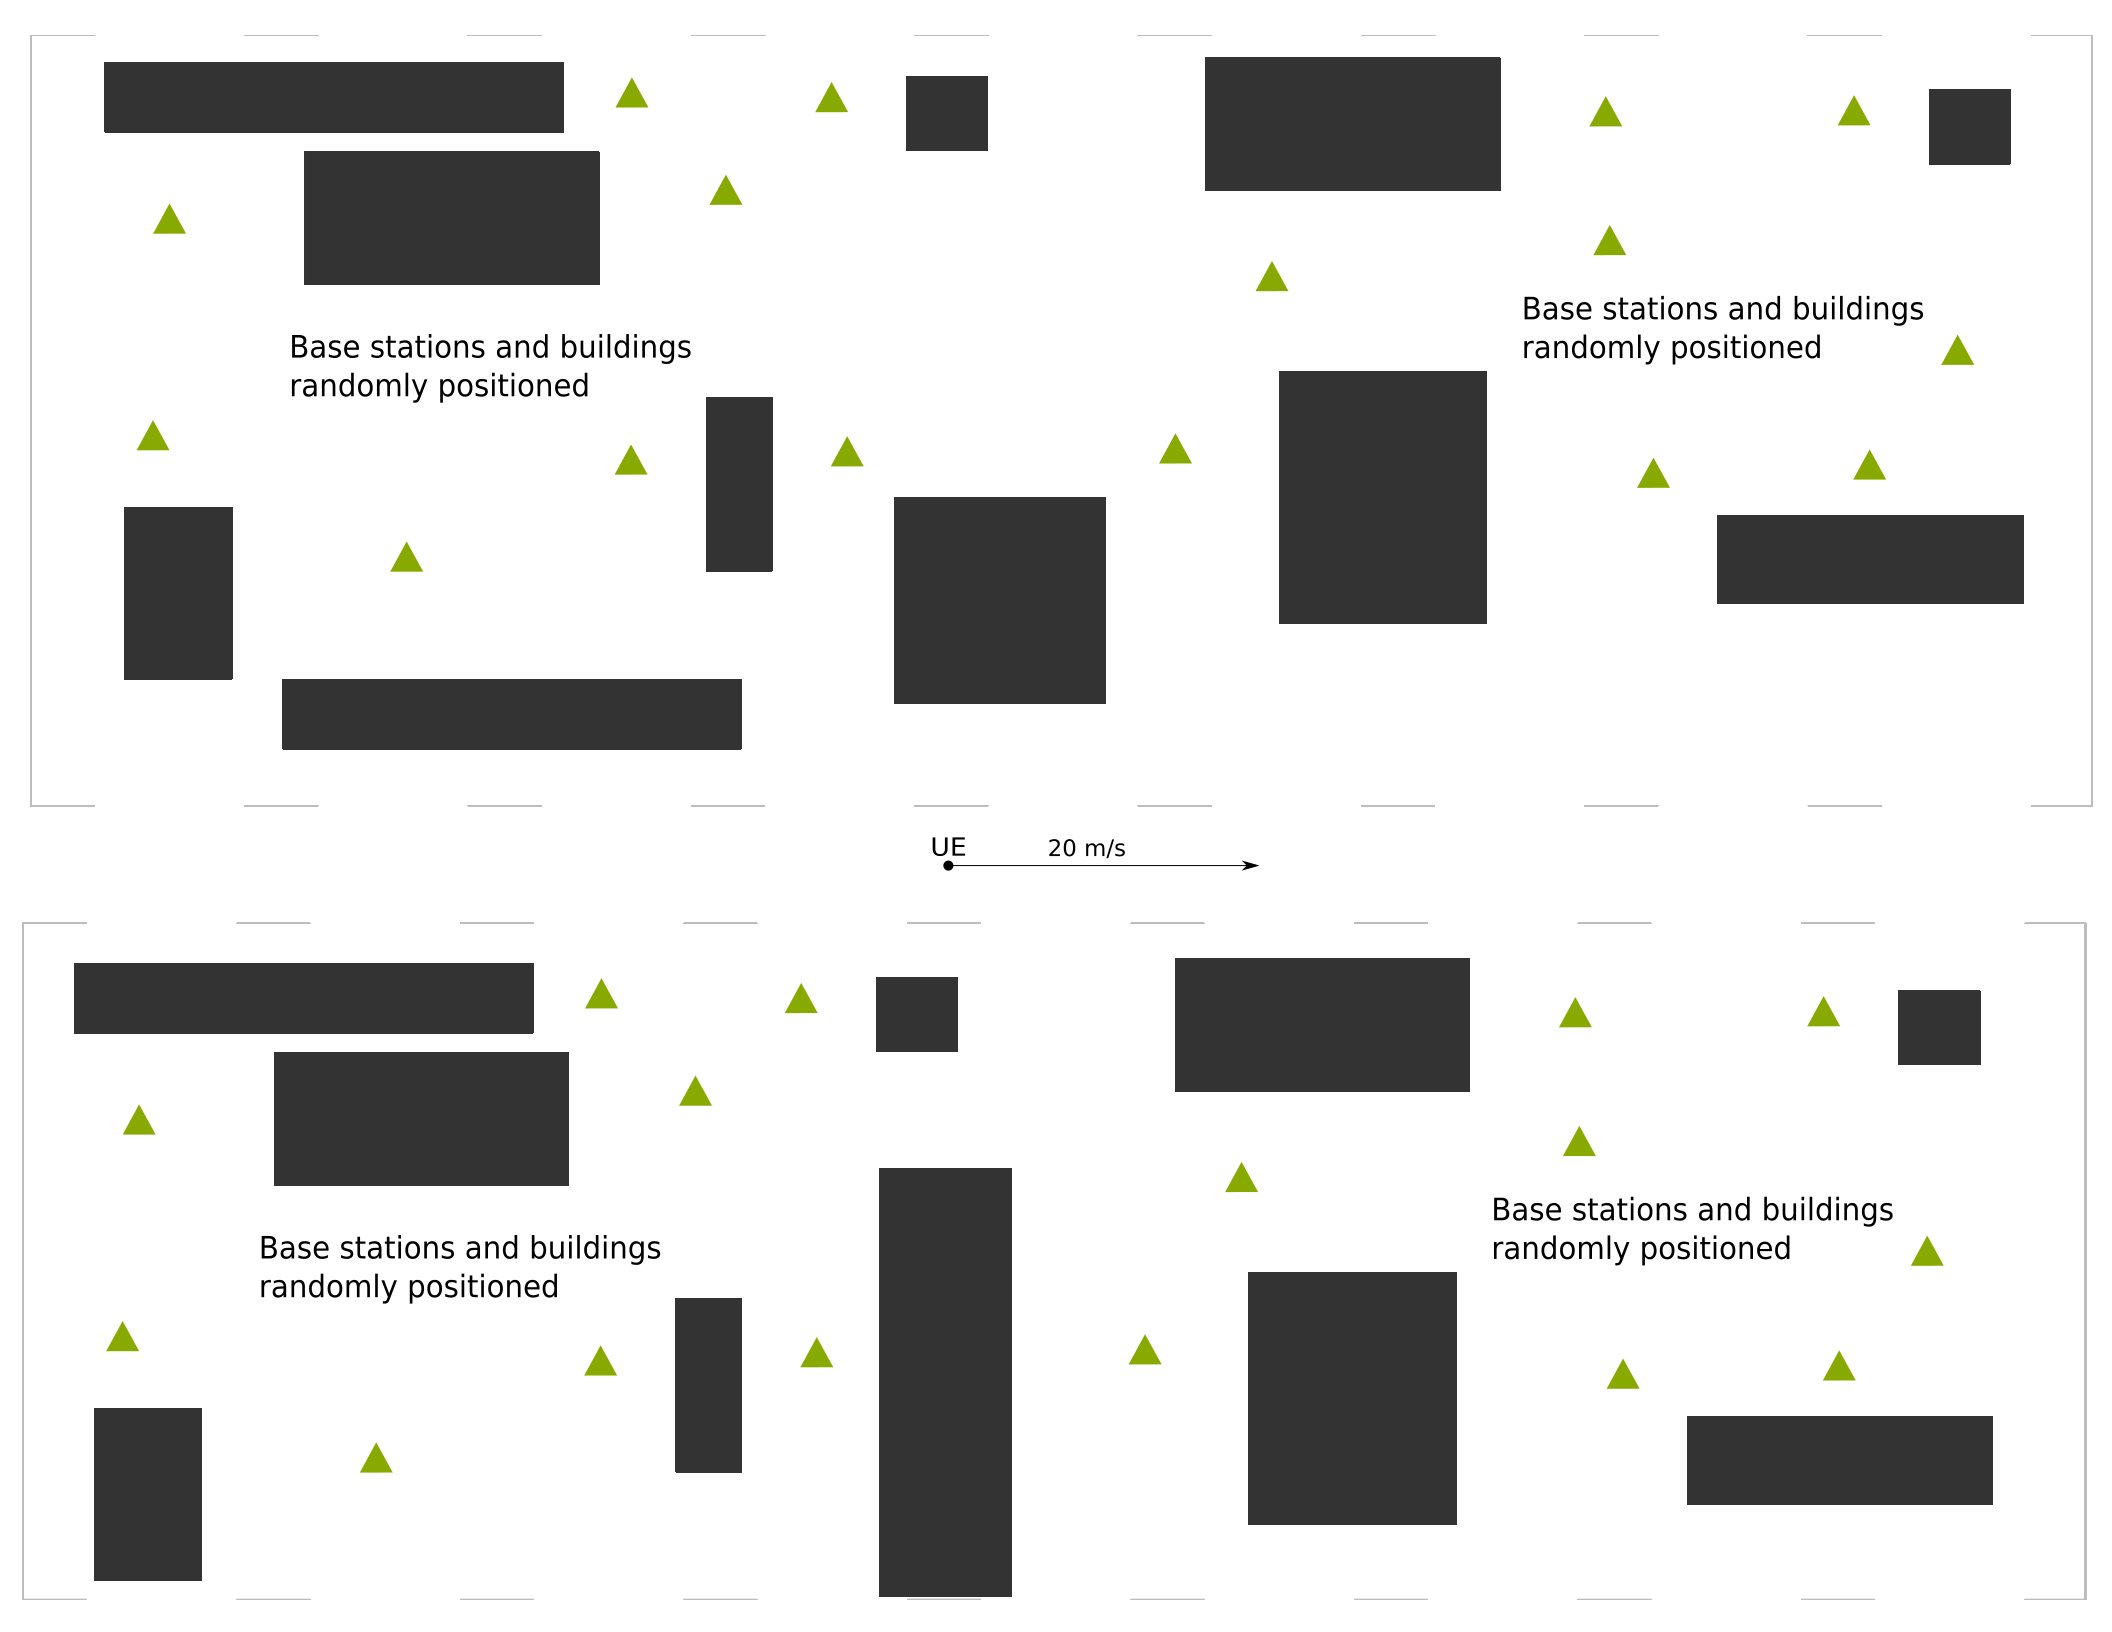
\includegraphics[scale=0.14]{scenario}
	% 		\caption{Example of an urban simulation scenario, base stations and buildings are generated randomly in the designated area.}
	% 	\end{figure}
	% \end{frame}

	\section{Results}

	\begin{frame}{Metrics analyzed}
		\begin{itemize}
			\item \textbf{Experienced throughput: } the throughput perceived by the user during the simulation \vspace{.5em}
			\item \textbf{PDCP latency: } the average latency of the only successfully received packets at the PDCP layer\vspace{.5em}
			\item \textbf{Packet Reception Ratio (PRR): } the number of correctly received packets divided by the total number of transmitted packets
		\end{itemize}
	\end{frame}

	\subsection{V2V Results}

	% \begin{frame}{V2V Results}
	% 	\begin{columns}
	% 		\column{0.5\textwidth}
	% 			\begin{figure}
	% 				\vspace{-0.2in}
	% 				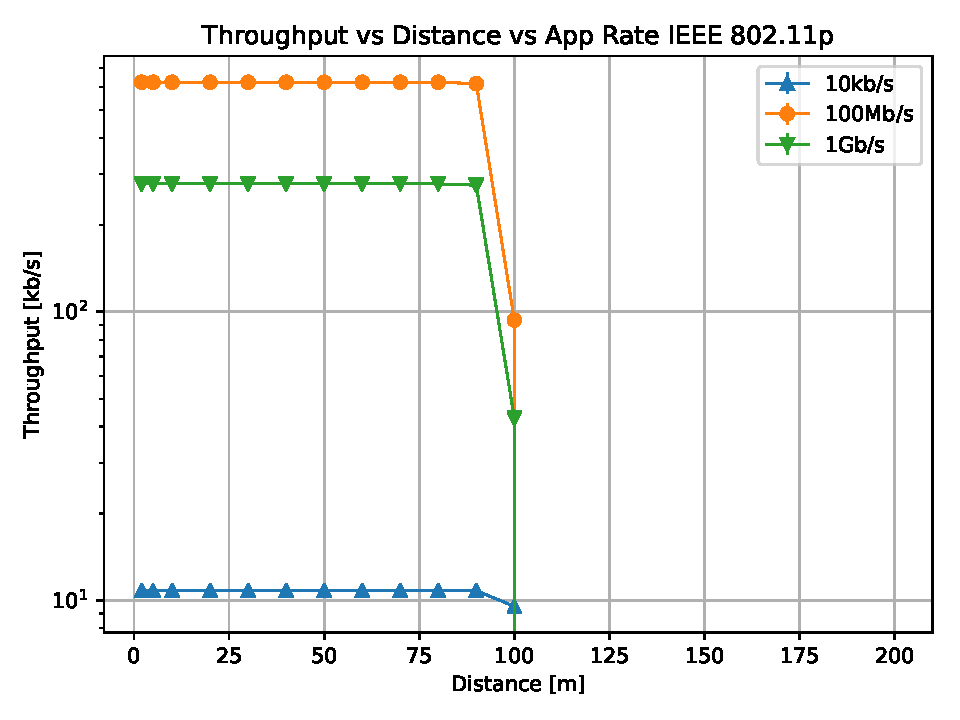
\includegraphics[scale=0.32]{throughput_distance_wave_UDP}
	% 			\end{figure}
	% 		\column{0.5\textwidth}
	% 			\begin{figure}
	% 				\vspace{-0.2in}
	% 				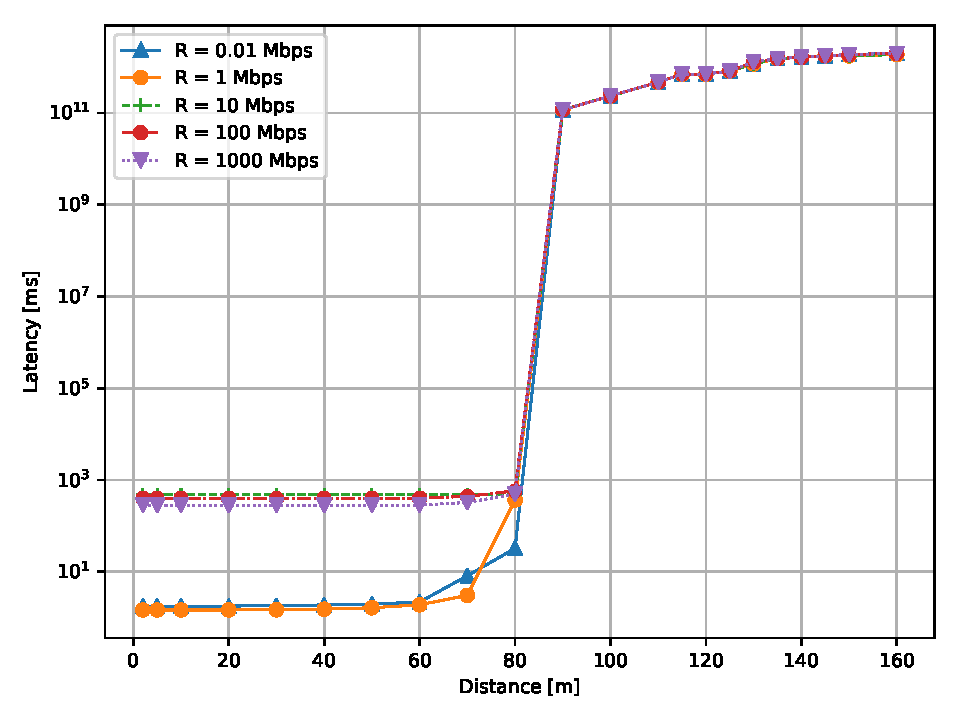
\includegraphics[scale=0.32]{latency_distance_wave_UDP}
	% 			\end{figure}
	% 			\begin{figure}
	% 				\vspace{-0.3in}
	% 				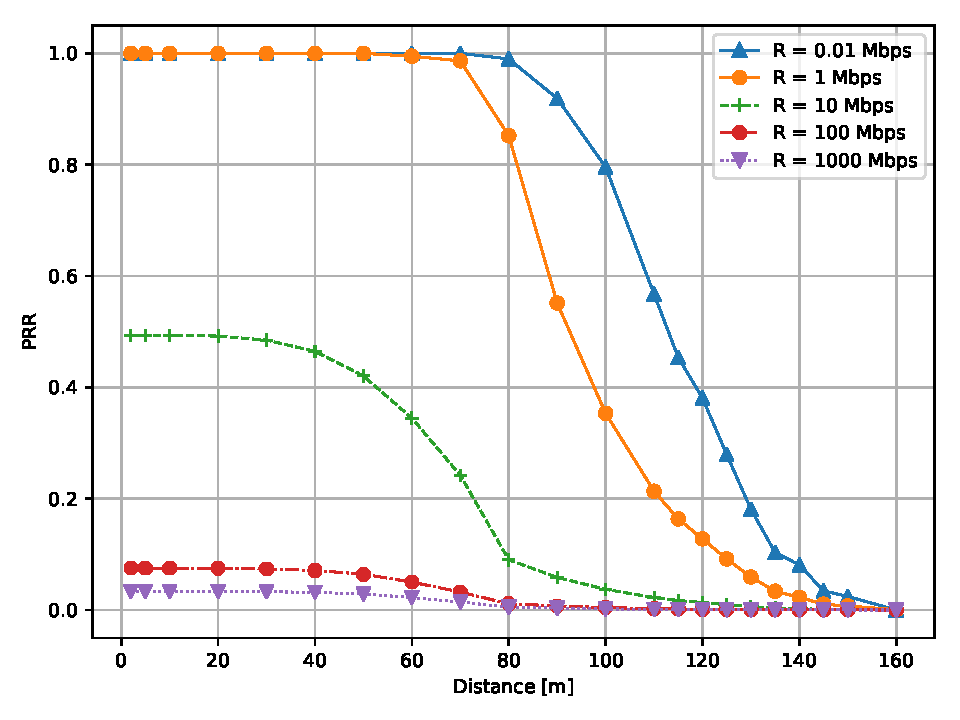
\includegraphics[scale=0.32]{PRR_distance_wave_UDP}
	% 			\end{figure}
	% 	\end{columns}
	% \end{frame}

	\begin{frame}{V2V Results - Throughput}
		\begin{figure}
			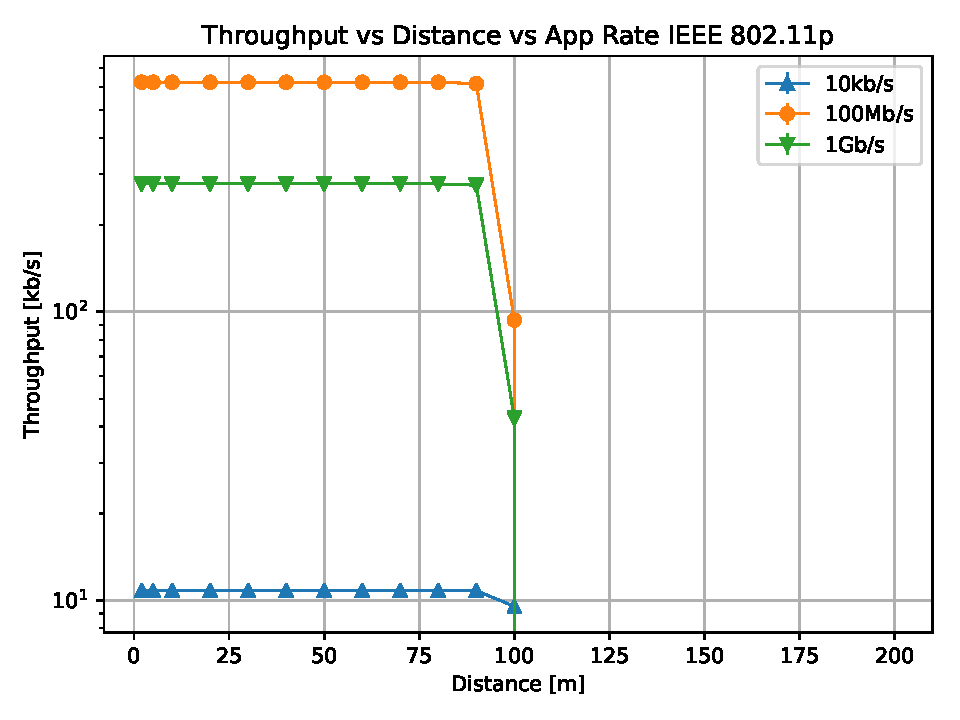
\includegraphics[scale=0.5]{throughput_distance_wave_UDP}
			\caption{Average throughput vs. inter-vehicle distance d for different values of the application rate R.}
		\end{figure}
	\end{frame}

	\begin{frame}{V2V Results - PRR}
		\begin{figure}
			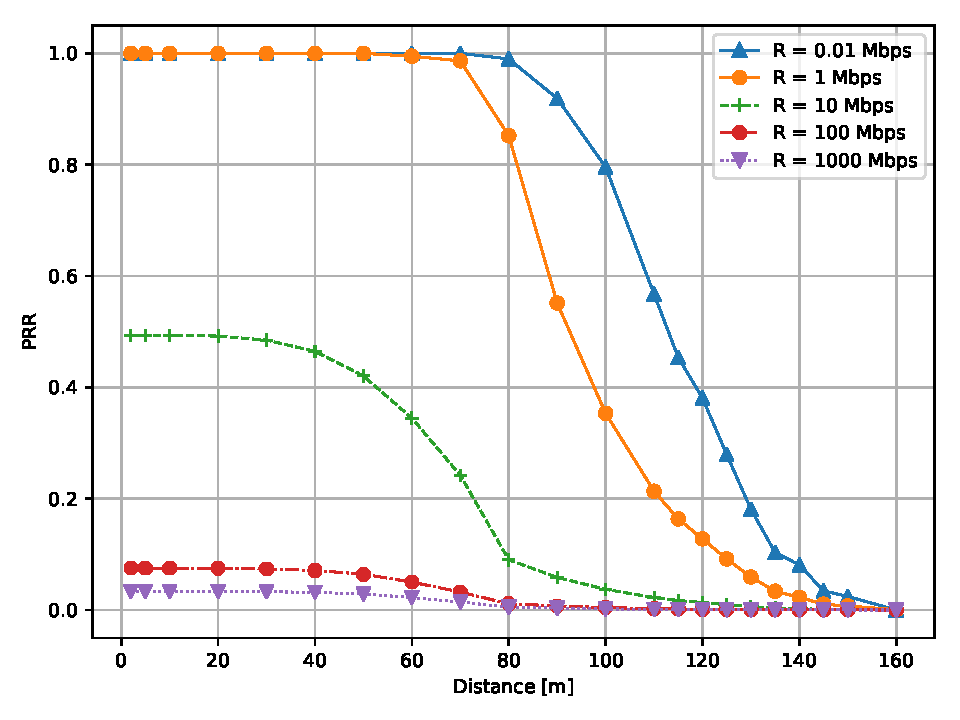
\includegraphics[scale=0.5]{PRR_distance_wave_UDP}
			\caption{PRR vs. inter-vehicle distance d for different values of the application rate R.}
		\end{figure}
	\end{frame}

	\begin{frame}{V2V Results - Latency}
		\begin{figure}
			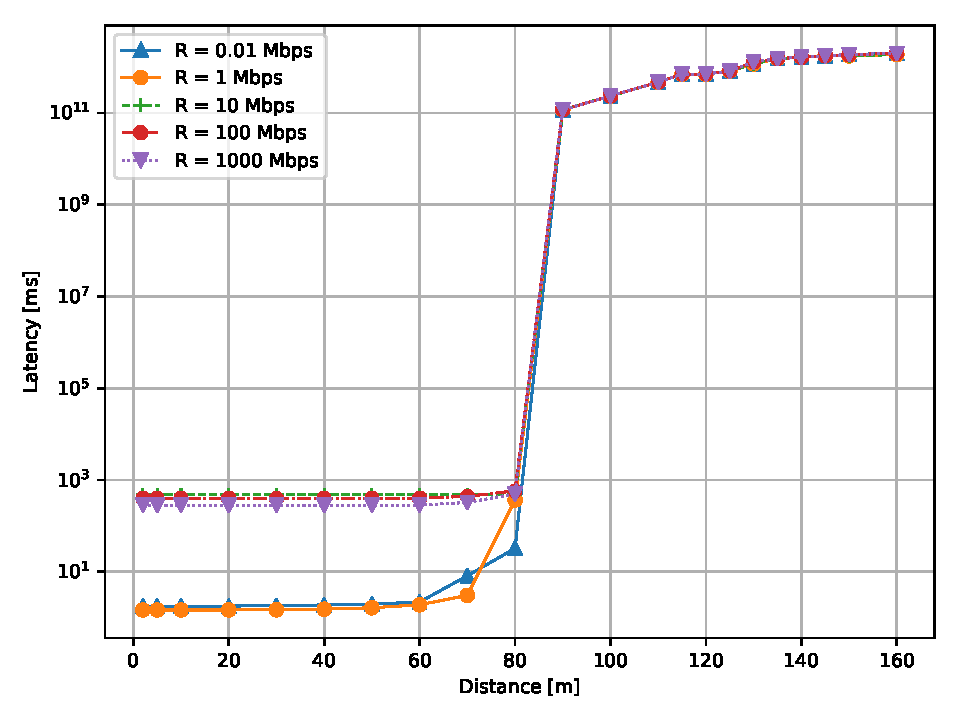
\includegraphics[scale=0.5]{latency_distance_wave_UDP}
			\caption{Average latency vs. inter-vehicle distance d for different values of the application rate R.}
		\end{figure}
	\end{frame}

	\subsection{V2I Results}

	% \begin{frame}{V2I results}
	% 	\begin{columns}
	% 		\column{0.5\textwidth}
	% 			\begin{figure}
	% 				\vspace{-0.2in}
	% 				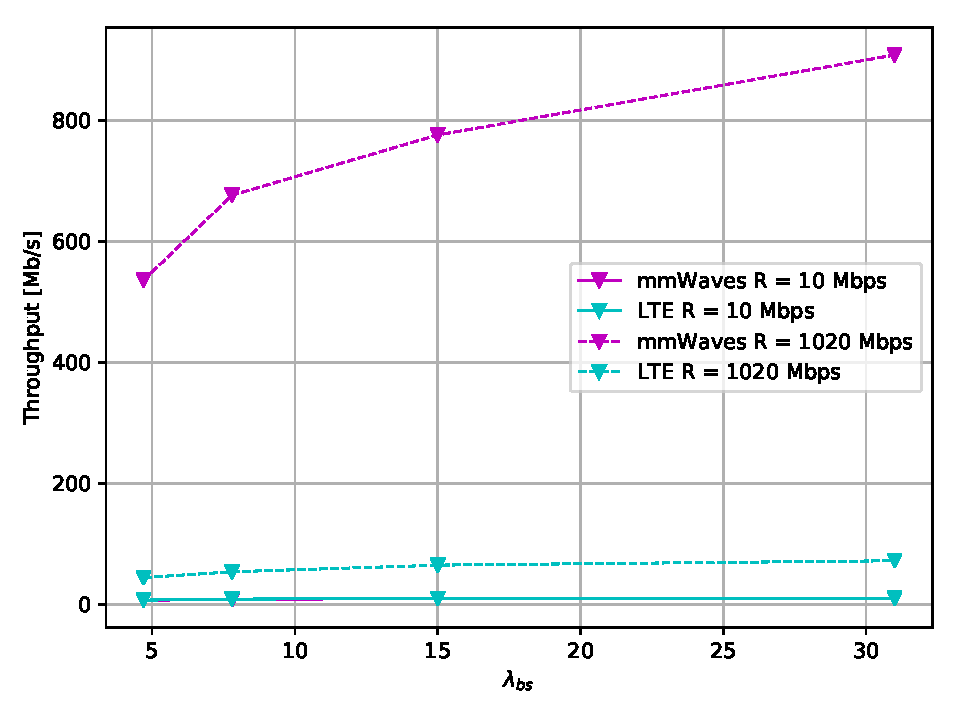
\includegraphics[scale=0.32]{throughput_random_lambda_bs_lte_mmwave_UDP}
	% 			\end{figure}
	% 			\column{0.5\textwidth}
	% 			\begin{figure}
	% 				\vspace{-0.1in}
	% 				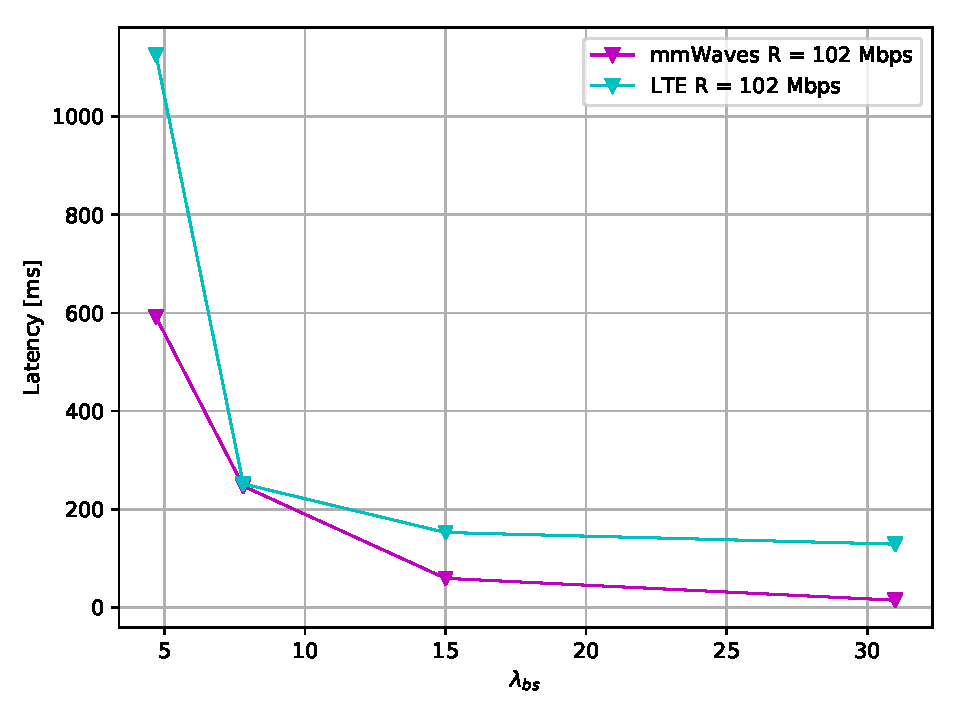
\includegraphics[scale=0.32]{latency_random_lambda_bs_lte_mmwave_UDP}
	% 			\end{figure}
	% 			\begin{figure}
	% 				\vspace{-0.3in}
	% 				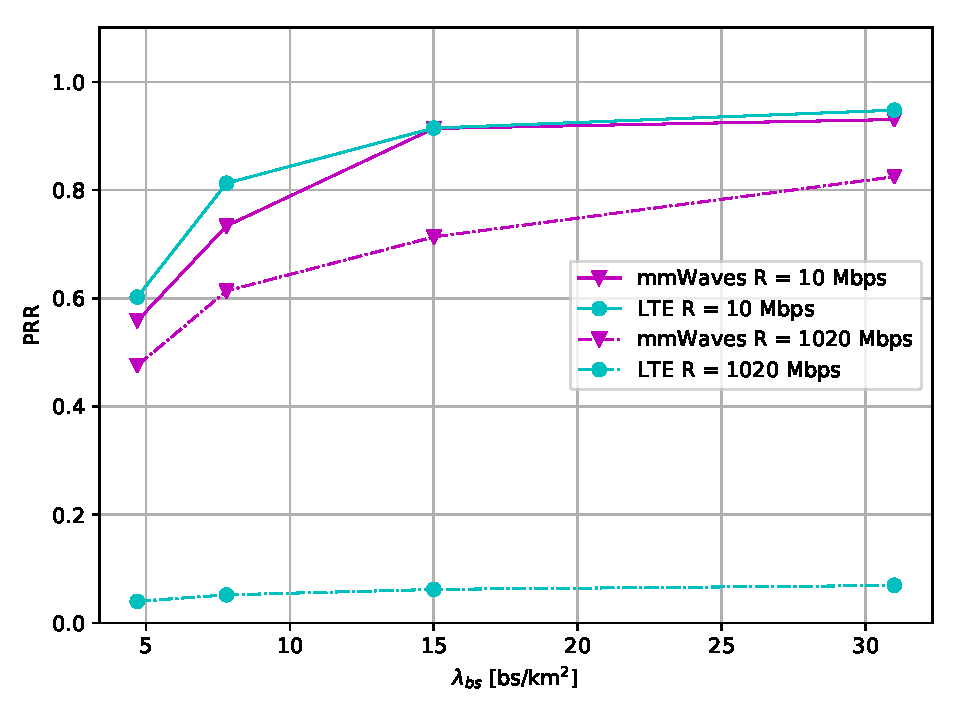
\includegraphics[scale=0.32]{PRR_random_lambda_bs_lte_mmwave_UDP}
	% 			\end{figure}
	% 	\end{columns}
	% \end{frame}

	\begin{frame}{V2I Results - Throughput}
		\begin{figure}
			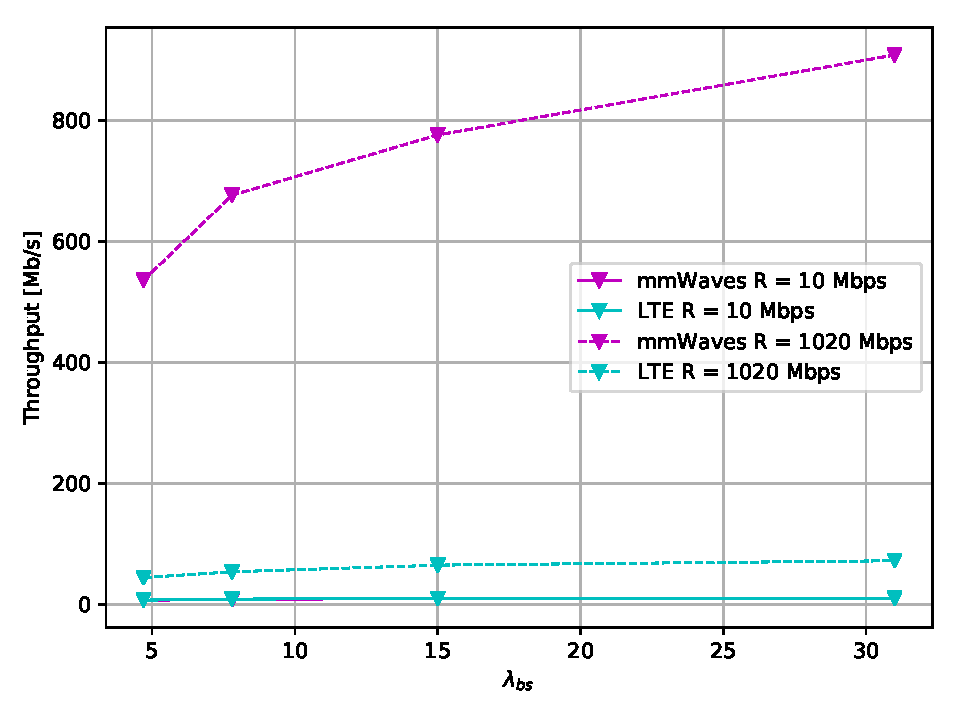
\includegraphics[scale=0.5]{throughput_random_lambda_bs_lte_mmwave_UDP}
			\caption{Throughput vs. base station density $\lambda_{bs}$ for different values of the application rate R.}
		\end{figure}
	\end{frame}

	\begin{frame}{V2I Results - PRR}
		\begin{figure}
			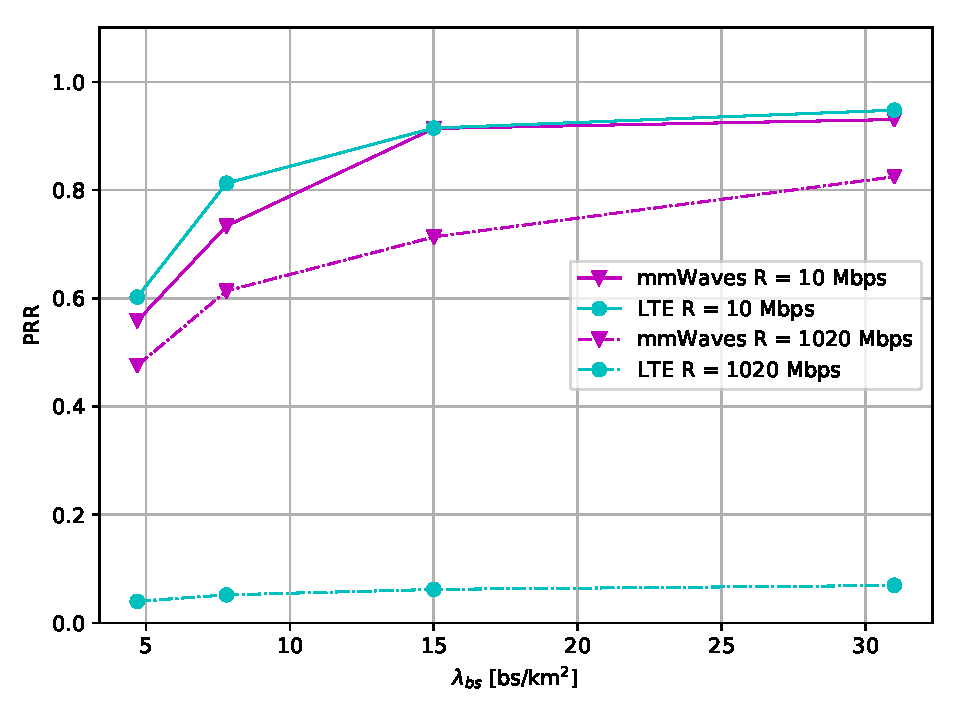
\includegraphics[scale=0.5]{PRR_random_lambda_bs_lte_mmwave_UDP}
			\caption{PRR vs. base station density $\lambda_{bs}$ for different values of the application rate R.}
		\end{figure}
	\end{frame}

	\begin{frame}{V2I Results - Latency}
		\begin{figure}
			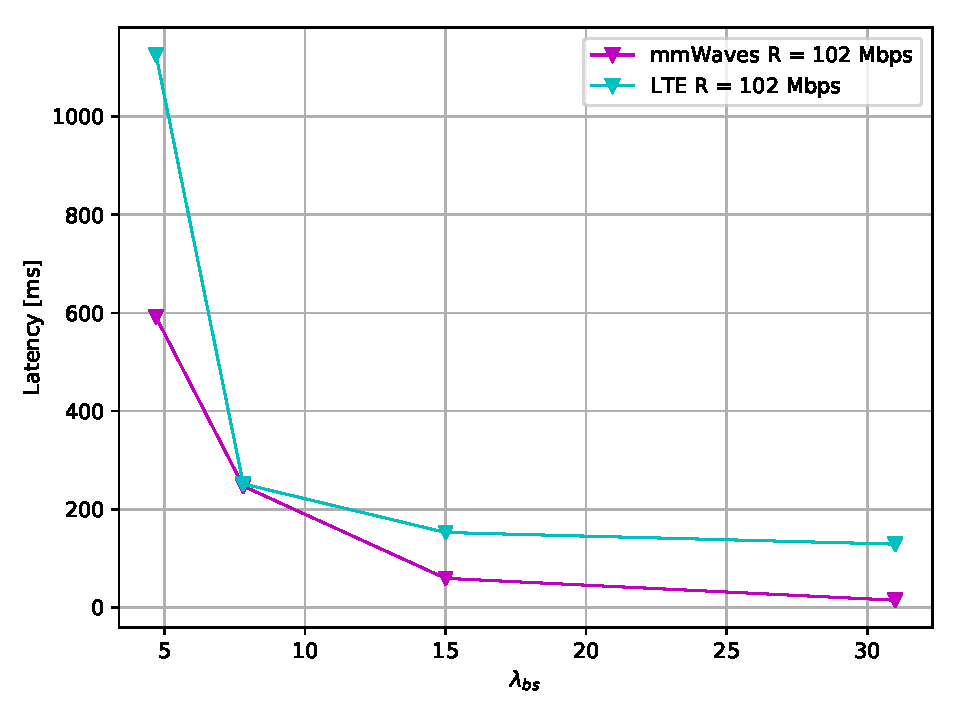
\includegraphics[scale=0.5]{latency_random_lambda_bs_lte_mmwave_UDP}
			\caption{Latency vs. base station density $\lambda_{bs}$ for different values of the application rate R.}
		\end{figure}
	\end{frame}

	\section{Conclusions}
	\begin{frame}{Conclusions}
		\textbf{IEEE 802.11p/WAVE}
		\begin{itemize}
			\item Low-rate and short-range connectivity
			\item Reliable communication and low latency
			\item Suitable for safety applications in 5G vehicular networks
		\end{itemize}
		\textbf{LTE}
		\begin{itemize}
			\item Good connectivity for datarates under 100 Mbps
			\item Capillar network of infrastructures available
			\item Suitable for some non-safety applications and as support technology
		\end{itemize}
		\textbf{mmWaves}
		\begin{itemize}
			\item High blockage sensitivity
			\item Extremely high throughput and low latency
			\item Suitable for the most demanding non-safety applications if supported by LTE
		\end{itemize}
	\end{frame}

	\begin{frame}{Acknowledgements}
		\center{\Large\textbf{Thank you for your attention!}}
	\end{frame}
\end{document}
